
\SbSSCT{Styles sans variable}{Styles without variable}

\begin{tabular}{|c|c|} \hline  
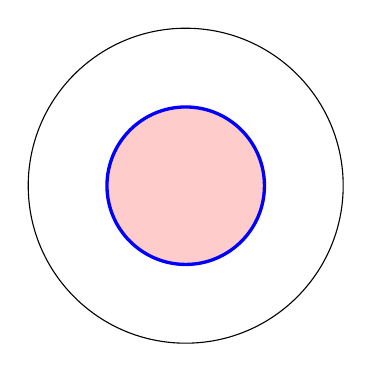
\begin{tikzpicture}[mon style/.style={draw=blue,fill=red!20,very thick},baseline=0pt]
\draw (0,0) circle (2cm);
\draw[mon style] (0,0) circle (1cm);
\end{tikzpicture}
&  
\parbox{10cm}{ 
\BS{begin}\AC{tikzpicture} [mon style/.\RDD{style}=\AC{draw=blue, fill=red!20, very thick}]\\
\BS{draw} (0,0) circle (2cm); \\
\BS{draw}[mon style] (0,0) circle (1cm); \\
\BS{end}\AC{tikzpicture} \\ } 
\\ \hline 
\end{tabular} 


\SbSSCT{Styles avec variable}{Styles with variable}

\begin{tabular}{|c|c|} \hline  

\begin{tikzpicture}[mon style/.style={draw=#1,thick,fill=#1!50,scale=.5}]
\filldraw [mon style=red] (0,0) rectangle (2,1);
\filldraw [mon style=blue] (3,0) rectangle (5,1);
\end{tikzpicture}
&  
\parbox{12cm}{ 
\BS{begin}\AC{tikzpicture} [mon style/.\RDD{style}=\AC{draw={\color{red}  \#1}, thick, fill={\color{red}  \#1}!50, scale=.5}]\\
\BS{filldraw} [mon style=red] (0,0) rectangle (2,1);\\
\BS{filldraw} [mon style=blue] (3,0) rectangle (5,1);\\
\BS{end}\AC{tikzpicture} \\ 
} 
\\ \hline   

\end{tabular} 




\begin{tabular}{|c|c|} \hline 
 \multicolumn{2}{|c|}{\TFRGB{valeur par défaut}{With a default value }}
 \\ \hline

\begin{tikzpicture}[mon style/.style={draw=#1,thick,fill=#1!50,scale=.5},
mon style/.default=black]
\filldraw [mon style] (0,0) rectangle (2,1);
\filldraw [mon style=blue] (3,0) rectangle (5,1);
\end{tikzpicture}
&  
\parbox{12cm}{ 
\BS{begin}\AC{tikzpicture} [mon style/.\RDD{style}=\AC{draw={\color{red}  \#1},fill={\color{red}  \#1}!20,very thick},\\
mon style/\RDD{default}=black] \\
\BS{filldraw} [mon style] (0,0) rectangle (2,1);\\
\BS{filldraw} [mon style=blue] (3,0) rectangle (5,1);\\
\BS{end}\AC{tikzpicture} }  
\\ \hline   

\end{tabular} 
